%%===========================================================%%
%%                                                           %%
%%                        CORRECTIONS                        %%
%%                                                           %%
%%===========================================================%%


\chapter{Corrections}\label{chap:corrections}

\section{Method of corrections application}
\begin{equation}
  \frac{d\sigma}{dq} = \frac{1}{\Delta q} \times \frac{1}{\varepsilon} \times \frac{N^{\mathit{w}}-N^{\mathit{w}}_\textrm{bkgd}}{\mathit{L}_{\textrm{int}}^{\textrm{eff}}}
\end{equation}

%remembed about accounting for RP trigger eff!!!
\begin{equation}\label{eq:effectiveLumi}
	\mathit{L}_{\textrm{int}}^{\textrm{eff}} = \sum\limits_{\textrm{run}}\mathit{L}_{\textrm{int}}^{\textrm{run}} \times \epsilon_{\textrm{veto}}(L^{\textrm{run}})
\end{equation}
% \left(\epsilon_{\textrm{veto}}^{\textrm{online}} \oplus \epsilon_{\textrm{veto}}^{\textrm{offline}}(L_{\textrm{run}}) \right)

\begin{equation}
	\varepsilon = \epsilon_{\textrm{\tiny ET/IT}} \times \epsilon_{\textrm{vrtx}}(q) \times \epsilon_{\ref{enum:CutZVx}} \times \epsilon_{\ref{enum:CutDeltaZVx}} \times \epsilon_{\ref{enum:CutMissingPt}} \times \epsilon_{\textrm{\tiny PID}}(q)
\end{equation}

\begin{equation}
	N^{\mathit{w}} = \sum\limits_{\textrm{event}}\mathit{w}_{\textrm{event}}
\end{equation}



\begin{equation}
	\mathit{w} = \left[\prod\limits_{\textrm{sign}} \epsilon_{\textrm{\tiny TOF}}(\textrm{sign}, \textrm{PID}, p_{T},z_{vx},\eta)  \times \prod\limits_{\textrm{sign}} \epsilon_{\textrm{\tiny TPC}}(\textrm{sign}, \textrm{PID}, p_{T},z_{vx},\eta) \times \prod\limits_{\textrm{side}}\epsilon_{\textrm{\tiny RP}}^{\textrm{side}}(p_{x},p_{y}) \right]^{-1},
\end{equation}
\[\textrm{sign}\in\{+,-\},~~\textrm{side}\in\{E,W\}\]
% ()

\section{Efficiencies and acceptances}
\subsection{Trigger efficiency}\label{sec:triggerEff}
\subsubsection{Online veto (BBC-small and ZDC veto)}
%---------------------------
\begin{figure}[ht!]
\centering%
\includegraphics[width=0.65\linewidth,page=1]{graphics/corrections/OnlineVetoEffVsInstLumi_graph.pdf}%
\caption{Overall efficiency of the online BBC-small and ZDC veto as a function of instantaneous luminosity.}\label{fig:onlineVetoEff}%
\end{figure}
%---------------------------
\subsubsection{RP triggering efficiency}
\subsubsection{Up and Down RP combination veto}
\subsection{Cuts efficiency}\label{sec:cutsEff}
\subsubsection{TPC \texorpdfstring{$z$}{z}-vertex cut~(\ref{enum:CutZVx})}
\subsubsection{TPC-RP \texorpdfstring{$z$}{z}-vertex matching~(\ref{enum:CutDeltaZVx})}
\subsubsection{Primary vertices limit~(\ref{enum:CutPrimVx}), BBC-large veto~(\ref{enum:CutBbcLarge}) and TOF clusters limit~(\ref{enum:CutTofClusters})}
%---------------------------
\begin{figure}[ht!]
\centering%
\includegraphics[width=0.65\linewidth,page=1]{graphics/corrections/OnlineAndOfflineVetoEffVsInstLumi_graph.pdf}%
\caption{Overall efficiency of the online BBC-small and ZDC veto, primary vertices limit~(\ref{enum:CutPrimVx}), BBC-large veto~(\ref{enum:CutBbcLarge}) and TOF clusters limit~(\ref{enum:CutTofClusters}) as a function of instantaneous luminosity.}\label{fig:onlineAndOfflineVetoEff}%
\end{figure}
%---------------------------
\subsubsection{Missing \texorpdfstring{$p_{T}$}{pT} cut~(\ref{enum:CutMissingPt})}
\subsubsection{Particle identification~(\ref{enum:CutPid})}

It is possible to transform dE/dx in MC to make it follow the shape of dE/dx in the data. 
We know that nSigmaX (where X=Pion, Kaon, Proton, ...) variable follows a gaussian distribution (for particle X)
 \[nSigmaX = \Big( \ln{\frac{dE/dx}{\langle dE/dx\rangle_{X}}} \Big) / \sigma_{dE/dx},~~~~~f(nSigmaX) = \mathcal{N}(nSigmaX; \mu=0,\sigma=1)\]
therefore $dE/dx$ itself follows log-normal distribution:
\[f(dE/dx) = \mathcal{L}og\mathcal{N}(dE/dx; \mu=\langle dE/dx\rangle,\sigma=\sigma_{dE/dx}) = \frac{1}{\sqrt{2\pi}\cdot \sigma\cdot dE/dx}e^{-\frac{\ln^{2}{\frac{dE/dx}{\langle dE/dx\rangle}}}{2\sigma^{2}}}\]
The transformation we want to apply should preserve the shape of $dE/dx$ (so that it is still described by $\mathcal{L}og\mathcal{N}$), however it should change $\mu$ and $\sigma$ so that these values are euqal to those seen in the data. The transformation that satisfies above postulate is
\[dE/dx' = c\cdot (dE/dx)^{a}\]
Parameters of the distribution $\mathcal{L}og\mathcal{N}(dE/dx')$ would be then
\[\mu' = c\cdot\mu^{a},~~~~\sigma' = a\cdot\sigma\]
From above we get formulae for parameters of the transformation:
\[a=\sigma'/\sigma,~~~~c = \frac{\mu'}{\mu^{a}}\]

AlternativeToCrystallBall~\cite{AlternativeToCrystallBall}~Eq.~\eqref{eq:expTail}

\begin{equation}\label{eq:expTail}
	f(dE/dx)=\left\{
                \begin{array}{ll}
                  \frac{A}{\sqrt{2\pi}\cdot \sigma\cdot dE/dx}\exp{\Bigg(-\frac{1}{2}\Big(\frac{\ln{\frac{dE/dx}{\langle dE/dx\rangle}}}{\sigma}\Big)^{2}\Bigg)} & \textrm{for}~\frac{\ln{\frac{dE/dx}{\langle dE/dx\rangle}}}{\sigma} \leq k \\
                  \frac{A}{\sqrt{2\pi}\cdot \sigma\cdot dE/dx}\exp{\Bigg(-k\cdot \frac{\ln{\frac{dE/dx}{\langle dE/dx\rangle}}}{\sigma} + \frac{1}{2}k^{2} - k^{-1}\left(\frac{\frac{\ln{\frac{dE/dx}{\langle dE/dx\rangle}}}{\sigma}}{k}-1\right)^{k} \Bigg)} & \textrm{for}~\frac{\ln{\frac{dE/dx}{\langle dE/dx\rangle}}}{\sigma} > k
                \end{array}
              \right.
\end{equation}



%---------------------------
\begin{figure}[hb]
\centering
\parbox{0.495\textwidth}{
  \centering
  \includegraphics[width=\linewidth,page=4]{graphics/corrections/dEdx_fitPerMomentumBin_3rdIteration.pdf}\\
  \includegraphics[width=\linewidth,page=14]{graphics/corrections/dEdx_fitPerMomentumBin_3rdIteration.pdf}\\
  \includegraphics[width=\linewidth,page=24]{graphics/corrections/dEdx_fitPerMomentumBin_3rdIteration.pdf}\\
  \includegraphics[width=\linewidth,page=34]{graphics/corrections/dEdx_fitPerMomentumBin_3rdIteration.pdf}
}~
\parbox{0.495\textwidth}{
  \centering
  \includegraphics[width=\linewidth,page=9]{graphics/corrections/dEdx_fitPerMomentumBin_3rdIteration.pdf}\\
  \includegraphics[width=\linewidth,page=19]{graphics/corrections/dEdx_fitPerMomentumBin_3rdIteration.pdf}\\
  \includegraphics[width=\linewidth,page=29]{graphics/corrections/dEdx_fitPerMomentumBin_3rdIteration.pdf}\\
  \includegraphics[width=\linewidth,page=39]{graphics/corrections/dEdx_fitPerMomentumBin_3rdIteration.pdf}
}%
\caption[Fits to dE/dx spectra from the data.]{Fits of sum of functions from Eq.~\eqref{eq:expTail} corresponding to different particle species to dE/dx spectra from the data in a few momentum bins.}\label{fig:dEdxFits}
\end{figure}
%---------------------------



%---------------------------
\begin{figure}[hb]
\centering
\parbox{0.4725\textwidth}{
  \centering
  \begin{subfigure}[b]{\linewidth}{
                \subcaptionbox{\label{fig:dEdxMeanOffsetMC}}{\includegraphics[width=\linewidth]{graphics/corrections/dEdxMeanOffset_allPIDs.pdf}\vspace*{-10pt}}}
  \end{subfigure}\\
  \begin{subfigure}[b]{\linewidth}\addtocounter{subfigure}{1}{
                \subcaptionbox{\label{fig:dEdxMeanOffsetData}}{\includegraphics[width=\linewidth]{graphics/corrections/dEdxMeanOffset_allPIDs_data.pdf}\vspace*{-10pt}}}
  \end{subfigure}
}
\quad
\parbox{0.4725\textwidth}{
  \centering
  \begin{subfigure}[b]{\linewidth}\addtocounter{subfigure}{-2}{
                \subcaptionbox{\label{fig:dEdxWidthMC}}{\includegraphics[width=\linewidth]{graphics/corrections/dEdxWidth_allPIDs.pdf}\vspace*{-10pt}}}
  \end{subfigure}\\
  \begin{subfigure}[b]{\linewidth}\addtocounter{subfigure}{1}{
                \subcaptionbox{\label{fig:dEdxWidthData}}{\includegraphics[width=\linewidth]{graphics/corrections/dEdxWidth_allPIDs_data.pdf}\vspace*{-10pt}}}
  \end{subfigure}
}%
\caption[Parameters of track dE/dx as a function of reconstructed momentum for a few particle species.]{Difference between MPV of dE/dx predicted by Bichsel parametrization and obtained from the fit of Eq.~\eqref{eq:expTail} to dE/dx distribution in the data (\ref{fig:dEdxMeanOffsetData}) and MC sample (\ref{fig:dEdxMeanOffsetMC}) and dE/dx width parameter in data (\ref{fig:dEdxWidthData}) and MC (\ref{fig:dEdxWidthMC}) as a function of reconstructed particle momentum for a few particle species. Solid lines represent fits to points of corresponding color.}\label{fig:dEdxParametersMC}
\end{figure}
%---------------------------


\begin{equation}\label{eq:dEdxParametrization}
	g(p) = P_{1} + P_{2}\cdot \exp{\left(-P_{3}\cdot p\right)} + P_{4}\cdot \arctan{\big(P_{5}\cdot(p-P_{6})\big)}
\end{equation}



\begin{table}[ht!]\centering%
\subcaptionbox{\label{tab:dEdxParametersMC}}{%
 \begin{tabular}{r||c|c|c|c|c|c||c|c|c|c|c|c}%\hline
 \multirow{2}{*}{\textbf{PID}} &  \multicolumn{6}{c||}{\bm{$\langle dE/dx\rangle_{\textrm{\textbf{Bichsel}}} - \langle dE/dx\rangle_{\textrm{\textbf{MC}}}$}} & \multicolumn{6}{c}{\bm{$\sigma(dE/dx)_{\textrm{\textbf{MC}}}$}} \\ \cline{2-13}
  & $P_{1}$ & $P_{2}$ & $P_{3}$ & $P_{4}$ & $P_{5}$ & $P_{6}$ & $P_{1}$ & $P_{2}$ & $P_{3}$ & $P_{4}$ & $P_{5}$ & $P_{6}$ \\ \Xhline{2\arrayrulewidth}
$\bm{\pi^{\pm}}$ &\scriptsize 3.618e-8 &\scriptsize 5.838e-9 &\scriptsize 5.481 &\scriptsize          &\scriptsize         &\scriptsize          &\scriptsize 0.0809 &\scriptsize -0.023 &\scriptsize 0.450 &\scriptsize -7.84e-3 &\scriptsize 1.8489 &\scriptsize 1.04 \\ \hline
$\bm{K^{\pm}}$ &\scriptsize -1.01e-10 &\scriptsize -9.983e-6 &\scriptsize 7.581 &\scriptsize          &\scriptsize         &\scriptsize         &\scriptsize 0.0628 &\scriptsize 0.022 &\scriptsize 5.381 &\scriptsize 3.06e-3 &\scriptsize 7.3070 &\scriptsize 0.547 \\ \hline
$\bm{p,\bar{p}}$ &\scriptsize -4.041e-8 &\scriptsize -1.179e-5 &\scriptsize 4.277 &\scriptsize          &\scriptsize         &\scriptsize         &\scriptsize 0.0660 &\scriptsize 0.082 &\scriptsize 12.042 &\scriptsize 1.07e-3 &\scriptsize 7.2872 &\scriptsize 0.889 \\ \hline
$\bm{e^{\pm}}$ &\scriptsize -1.542e-7 &\scriptsize 3.393e-7 &\scriptsize 5.025 &\scriptsize          &\scriptsize         &\scriptsize           &\scriptsize 0.0572 &\scriptsize 0.982 &\scriptsize 37.984 &\scriptsize 2.61e-3 &\scriptsize -27.995 &\scriptsize 0.693 \\ \hline
$\bm{d,\bar{d}}$ &\scriptsize -2.469e-6 &\scriptsize 0.3706 &\scriptsize 21.654 &\scriptsize 5.131e-7 &\scriptsize 30.050 &\scriptsize 0.781      &\scriptsize 0.1311 &\scriptsize -0.971 &\scriptsize 4.691 &\scriptsize          &\scriptsize         &\scriptsize         
\end{tabular}%
}\newline\centering%
\subcaptionbox{\label{tab:dEdxParametersData}}{%
\begin{tabular}{r||c|c|c|c|c|c||c|c|c|c|c|c}%\hline
 \multirow{2}{*}{\textbf{PID}} &  \multicolumn{6}{c||}{\bm{$\langle dE/dx\rangle_{\textrm{\textbf{Bichsel}}} - \langle dE/dx\rangle_{\textrm{\textbf{Data}}}$}} & \multicolumn{6}{c}{\bm{$\sigma(dE/dx)_{\textrm{\textbf{Data}}}$}} \\ \cline{2-13}
  & $P_{1}$ & $P_{2}$ & $P_{3}$ & $P_{4}$ & $P_{5}$ & $P_{6}$ & $P_{1}$ & $P_{2}$ & $P_{3}$ & $P_{4}$ & $P_{5}$ & $P_{6}$ \\ \Xhline{2\arrayrulewidth}
 $\bm{\pi^{\pm}}$ & \scriptsize-1.236e-8 & \scriptsize1.777e-7 & \scriptsize9.938 & \scriptsize& \scriptsize& \scriptsize& \scriptsize0.0738 & \scriptsize16.86 & \scriptsize39.44 & \hspace*{-3pt}\scriptsize-1.704e-3\hspace*{-2pt} & \scriptsize~6.482~ & \scriptsize0.628\\ \hline
 $\bm{K^{\pm}}$ & \scriptsize5.49e-10 & \scriptsize-2.732e-6 & \scriptsize7.712 & \scriptsize& \scriptsize& \scriptsize& \scriptsize0.0743 & \hspace*{-2pt}\scriptsize2.67e-5\hspace*{-2pt} & \scriptsize7.17089 & \scriptsize& \scriptsize& \scriptsize\\ \hline
 $\bm{p,\bar{p}}$ & \scriptsize-2.140e-7 & \scriptsize0.0421 & \scriptsize48.305 & \scriptsize7.512e-8 & \scriptsize15.544 & \scriptsize0.575 & \scriptsize0.0779 & \scriptsize1.822 & \scriptsize22.4277 & \scriptsize& \scriptsize& \scriptsize\\ \hline
 $\bm{e^{\pm}}$ & \scriptsize6.701e-8 & \scriptsize3.304e-7 & \scriptsize7.845 & \scriptsize& \scriptsize& \scriptsize& \scriptsize0.0678 & \scriptsize468.9 & \scriptsize59.4001 & \scriptsize& \scriptsize& \scriptsize\\ \hline
 $\bm{d,\bar{d}}$ & \scriptsize-1.631e-7 & \scriptsize0.0818 & \scriptsize18.91 & \scriptsize& \scriptsize& \scriptsize& \scriptsize0.1259 & \scriptsize-0.288 & \scriptsize3.28733 & \scriptsize& \scriptsize& \scriptsize%\\ \hline
\end{tabular}
}\caption[Parameters of functions from Fig.~\ref{fig:dEdxParametersMC} describing track dE/dx as a function of reconstructed momentum for a few particle species (STARsim MC).]{Parameters of functions from Fig.~\ref{fig:dEdxParametersMC} describing track dE/dx as a function of reconstructed momentum for a few particle species. Units of parameters $P_{i}$ are such that if one provides momentum in Eq.~\eqref{eq:dEdxParametrization} in GeV/$c$ the resultant offset of dE/dx MPV with respect to Bichsel parametrization is in GeV/cm, and the resultant $\sigma$ parameter is unitless.}%\label{tab:dEdxParametersMC}
\end{table}




%---------------------------
\begin{figure}[hb]
\centering
\parbox{0.495\textwidth}{
  \centering
  \includegraphics[width=\linewidth,page=4]{graphics/corrections/dEdx_DataVsMC.pdf}\\
  \includegraphics[width=\linewidth,page=14]{graphics/corrections/dEdx_DataVsMC.pdf}\\
  \includegraphics[width=\linewidth,page=24]{graphics/corrections/dEdx_DataVsMC.pdf}\\
  \includegraphics[width=\linewidth,page=34]{graphics/corrections/dEdx_DataVsMC.pdf}
}~
\parbox{0.495\textwidth}{
  \centering
  \includegraphics[width=\linewidth,page=9]{graphics/corrections/dEdx_DataVsMC.pdf}\\
  \includegraphics[width=\linewidth,page=19]{graphics/corrections/dEdx_DataVsMC.pdf}\\
  \includegraphics[width=\linewidth,page=29]{graphics/corrections/dEdx_DataVsMC.pdf}\\
  \includegraphics[width=\linewidth,page=39]{graphics/corrections/dEdx_DataVsMC.pdf}
}%
\caption[Comparison of dE/dx spectra between data and MC.]{Comparison of the dE/dx spectra between the data and MC (before and after correction) in a few momentum bins.}\label{fig:dEdxDataVsMC}
\end{figure}
%---------------------------








%---------------------------
\begin{figure}[ht!]
\centering
\parbox{0.315\textwidth}{
  \centering
  \begin{subfigure}[b]{\linewidth}{
                \subcaptionbox{\label{fig:sqMassTof_DataVsMC_pion}}{\includegraphics[width=\linewidth,page=1]{graphics/corrections/sqMassTof_DataVsMC.pdf}}}
  \end{subfigure}
}
\quad
\parbox{0.315\textwidth}{
  \centering
  \begin{subfigure}[b]{\linewidth}{
                \subcaptionbox{\label{fig:sqMassTof_DataVsMC_kaon}}{\includegraphics[width=\linewidth,page=2]{graphics/corrections/sqMassTof_DataVsMC.pdf}}}
  \end{subfigure}
}
\quad
\parbox{0.315\textwidth}{
  \centering
  \begin{subfigure}[b]{\linewidth}{
                \subcaptionbox{\label{fig:sqMassTof_DataVsMC_proton}}{\includegraphics[width=\linewidth,page=3]{graphics/corrections/sqMassTof_DataVsMC.pdf}}}
  \end{subfigure}
}%
\caption{Comparison of $m^{2}$ from TOF between data and MC for exclusive $\pi^{+}\pi^{-}$, $K^{+}K^{-}$ and $p\bar{p}$.}
\end{figure}
%---------------------------









\subsection{RP track acceptance and reconstruction efficiency}\label{sec:rpAccAndEff}
\subsection{TPC track acceptance and reconstruction efficiency}\label{sec:tpcAccAndEff}

We define joint acceptance and efficiency of the reconstruction of a track in the TPC, $\epsilon_{\textrm{\tiny TPC}}$, as the probability that particle from the primary interaction generates signal in the detector which is reconstructed as a track that satisfies all quality criteria and whose $p_{T}$ and $\eta$ are within the kinematic region of the measurement (cut~\ref{enum:TpcQualityCuts}).

Thechnically this quantity is derived from STARsim MC embedded into zero-bias triggers in the following procedure:
\begin{enumerate}
	\item True-level primary particles of given ID and charge, with all physics ($p_{T}^{\textrm{true}}$, $\eta^{\textrm{true}}$) and detector ($z_{\textrm{vx}}$) quantities within defined region of the measurement, are selected ($set~A$).
	\item Each particle from $set~A$ is checked if global TPC track with more than half of hit points generated by this particle, was reconstructed. All global tracks which are associated with true-level primary particles and satisfy all criteria~\ref{enum:TpcQualityCuts} (except DCA(R) and DCA(z) which are not verified), form $set~B$.
	\item The joint TPC acceptance and efficiency is calculated as the ratio of the histograms of true-level quantities (such as $p_{T}$, $\eta$, $z_{\textrm{vx}}$) for particles from $set~B$ and particles from $set~A$:
	\begin{equation}\label{eq:tpcAccAndEffDefinition}
		\epsilon_{\textrm{\tiny TPC}}\left(p_{T}, \eta, z_{vx};~\textrm{sign},\textrm{PID}\right) = \frac{(p_{T},\eta, z_{vx})~\textrm{histogram for particles of given sign and ID from}~set~B}{(p_{T},\eta, z_{vx})~\textrm{histogram for particles of given sign and ID from}~set~A}.
	\end{equation}

\end{enumerate}

\subsection{TOF acceptance, reconstruction and track-matching efficiency}\label{sec:tofAccAndEff}

Combined TOF acceptance, hit reconstruction efficiency and matching efficiency with TPC tracks, $\epsilon_{\textrm{\tiny TOF}}$, is defined as the probability that the global TPC track that satisfy all criteria~\ref{enum:TpcQualityCuts} (except DCA(R) and DCA(z) which are not verified) is matched with hit in TOF (matching flag of the track is different from 0). This quantity is generally referred as ``TOF efficiency''.

It is calculated in two ways. In the first approach the STARsim MC embedded into zero-bias triggers is used. Tracks belonging to $set~B$ from Sec.~\ref{sec:tpcAccAndEff} are utilized. From these tracks a sub-sample of tracks with non-zero TOF matching flag is extracted ($set~C$). The TOF efficiency is calculated as
\begin{equation}\label{eq:tofAccAndEffDefinition}
		\epsilon_{\textrm{\tiny TOF}}\left(p_{T}, \eta, z_{vx};~\textrm{sign},\textrm{PID}\right) = \frac{(p_{T},\eta, z_{vx})~\textrm{histogram for particles of given sign and ID from}~set~C}{(p_{T},\eta, z_{vx})~\textrm{histogram for particles of given sign and ID from}~set~B}.
	\end{equation}

\subsection{TPC vertex reconstruction efficiency}\label{sec:tpcVxRecoEff}

The definition of vertex reconstruction efficiency established in this analysis is the probability that two global tracks, both associated with true-level primary particles from the kinematic region of the measurement, both satisfying all criteria~\ref{enum:TpcQualityCuts} (except DCA(R) and DCA(z) which are not verified) and both matched with hits in TOF, form a vertex listed in the collection of reconstructed primary vertices and DCA(R) and DCA(z) of both global tracks calculated w.r.t. this vertex is contained within the limits of cut~\ref{enum:TpcQualityCuts}.

\section{Particle energy loss}\label{sec:energyLoss}
\section{Background subtraction}\label{sec:bkgdSubtraction}
\section{Unfolding}\label{sec:unfolding}

% 
%   W analizie CEP wydajność werteksowania to prawdopodobieństwo że
%  oba pierwotne ślady z punktu B tworzą werteks (to znaczy są na liście
%  śladów primary wspólnego werteksu i spełniaja ciecia DCA).
%  Nie patrzymy na dodatkowe werteksy, hity w TOF, BBC_small
% 
% E) --- pozostałe wydajności
% 
%   w przypadku analizy CEP jest to pile-up czyli dodatkowy werteks lub
%   dodatkowy hit w TOF lub sygnał w BBC. Te poprawk mamy z embeddingu
%   patrząc ile przypadków z D ma dodatkowy werteks, hist w TOF lub BBC
% 
%   To samo powinniśmy dostać z analizy "naszych" zero-bias.
% 
%   W przypadku analizy SD mamy pile-up czyli dodatkowy werteks, BBC
%   po stronie protonu też to znamy z embeddingu lub "naszych" zero-bias.
% 
%   Dodatkowo dochodzą dodatkowe werteksy z oddziaływań wtórnych/rozpadów.
%   Ten efekt znamy z MC. Powinno być to samo z pile-up'em jak i  bez
% 
% 
% Jakieś uwagi?
